% Options for packages loaded elsewhere
\PassOptionsToPackage{unicode}{hyperref}
\PassOptionsToPackage{hyphens}{url}
%
\documentclass[
]{article}
\usepackage{amsmath,amssymb}
\usepackage{iftex}
\ifPDFTeX
  \usepackage[T1]{fontenc}
  \usepackage[utf8]{inputenc}
  \usepackage{textcomp} % provide euro and other symbols
\else % if luatex or xetex
  \usepackage{unicode-math} % this also loads fontspec
  \defaultfontfeatures{Scale=MatchLowercase}
  \defaultfontfeatures[\rmfamily]{Ligatures=TeX,Scale=1}
\fi
\usepackage{lmodern}
\ifPDFTeX\else
  % xetex/luatex font selection
\fi
% Use upquote if available, for straight quotes in verbatim environments
\IfFileExists{upquote.sty}{\usepackage{upquote}}{}
\IfFileExists{microtype.sty}{% use microtype if available
  \usepackage[]{microtype}
  \UseMicrotypeSet[protrusion]{basicmath} % disable protrusion for tt fonts
}{}
\makeatletter
\@ifundefined{KOMAClassName}{% if non-KOMA class
  \IfFileExists{parskip.sty}{%
    \usepackage{parskip}
  }{% else
    \setlength{\parindent}{0pt}
    \setlength{\parskip}{6pt plus 2pt minus 1pt}}
}{% if KOMA class
  \KOMAoptions{parskip=half}}
\makeatother
\usepackage{xcolor}
\usepackage{graphicx}
\makeatletter
\def\maxwidth{\ifdim\Gin@nat@width>\linewidth\linewidth\else\Gin@nat@width\fi}
\def\maxheight{\ifdim\Gin@nat@height>\textheight\textheight\else\Gin@nat@height\fi}
\makeatother
% Scale images if necessary, so that they will not overflow the page
% margins by default, and it is still possible to overwrite the defaults
% using explicit options in \includegraphics[width, height, ...]{}
\setkeys{Gin}{width=\maxwidth,height=\maxheight,keepaspectratio}
% Set default figure placement to htbp
\makeatletter
\def\fps@figure{htbp}
\makeatother
\setlength{\emergencystretch}{3em} % prevent overfull lines
\providecommand{\tightlist}{%
  \setlength{\itemsep}{0pt}\setlength{\parskip}{0pt}}
\setcounter{secnumdepth}{-\maxdimen} % remove section numbering
\ifLuaTeX
  \usepackage{selnolig}  % disable illegal ligatures
\fi
\IfFileExists{bookmark.sty}{\usepackage{bookmark}}{\usepackage{hyperref}}
\IfFileExists{xurl.sty}{\usepackage{xurl}}{} % add URL line breaks if available
\urlstyle{same}
\hypersetup{
  hidelinks,
  pdfcreator={LaTeX via pandoc}}

\author{}
\date{}

\begin{document}

\hypertarget{algorithms-description}{%
\subsection{1. Algorithms description}\label{algorithms-description}}

\hypertarget{muon-optimizer}{%
\subsubsection{1. Muon optimizer}\label{muon-optimizer}}

Muon (MomentUm Orthogonalized by Newton--Schulz) is an optimizer
designed for 2D parameter matrices. It first computes a standard SGD
with momentum update and then applies a post-processing step based on
the Newton--Schulz (NS) iteration to approximately orthogonalize the
update matrix. As a result, the update is effectively replaced by its
nearest semi-orthogonal counterpart, which improves the conditioning of
the update and amplifies underrepresented directions.

Compared to alternative orthogonalization methods, NS iteration provides
a favorable trade-off between numerical stability and efficiency. In
particular, it can be stably computed in bfloat16 precision and requires
only a small number of iterations (typically 3--5), making it
significantly faster than SVD-based approaches.

In terms of resource requirements, Muon inherits the same memory
footprint as SGD with momentum. The additional computational cost comes
from the NS iteration: for an \(n \times m\) parameter matrix (assuming
\(n \ge m\)), each iteration requires approximately\\
\(2(2nm^2 + m^3)\) FLOPs, which is upper-bounded by \(6nm^2\).

Thus, for \(T\) NS iterations, the total overhead is
\(\mathcal(6\cdot T \cdot nm^2)\), which in practice results in less
than 1\% additional FLOPs in typical transformer training regimes.

As a limitation, Muon is applicable only to 2D (and higher-dimensional
reshaped) weight matrices, and is not recommended for input/output
layers such as embeddings and final classifier heads, where different
optimization dynamics are empirically more effective. \#\#\# 2. AdamW
optimizer AdamW is an adaptive optimization algorithm based on Adam,
which maintains exponentially decaying estimates of first and second
moments of gradients. These moment estimates are used to compute
parameter-wise adaptive learning rates, improving convergence speed and
stability, especially in large-scale and sparse settings.

The key distinction of AdamW from the original Adam lies in decoupled
weight decay. Instead of incorporating L2 regularization into the
gradient, AdamW applies weight decay directly to the parameters during
the update step. This separation leads to better generalization and more
predictable regularization behavior.

In terms of computational cost, AdamW requires maintaining two
additional tensors per parameter (for first and second moments),
resulting in higher memory usage compared to SGD. Each update involves
element-wise operations, making it efficient on modern hardware, though
typically more expensive than SGD in both memory and compute.

AdamW is widely used as a strong baseline for training transformer
models and is particularly effective for optimizing embeddings,
normalization layers, and output heads, where adaptive scaling of
updates is beneficial. \#\# 2. Performance comparison \#\#\# 1. Data,
model and experiment setup To compare the optimizers, we used the
pretrained model
\href{https://huggingface.co/Qwen/Qwen2.5-0.5B}{Qwen2.5-0.5B}, which was
fine-tuned on the
\href{https://huggingface.co/datasets/Elriggs/openwebtext-100k}{openwebtext-100k}
dataset.

An initial analysis of the dataset showed that the median sequence
length is approximately 673 tokens. To efficiently utilize available
VRAM while preserving semantic coherence, we employed sequence packing
with document boundaries separated by the EOS token and used a fixed
sequence length of 1024 tokens. This setup allows for higher token
utilization per batch while minimizing fragmentation of individual
documents.

Training was performed using deterministic settings (fixed seeds) to
ensure comparability across runs. A total of three experiments were
conducted, differing primarily in:\\
-effective batch size (fixed segment length, maximized batch size, tuned
gradient accumulation steps),\\
-Muon learning rate,\\
-Muon weight decay.

All other hyperparameters (model, tokenizer, scheduler, sequence length,
and data pipeline) were kept constant to isolate the effect of the
optimizer configuration.

Each model was trained for one full pass over the dataset. After
training, models were evaluated on a set of standard language
understanding benchmarks: PIQA, ARC-Easy, ARC-Challenge, Winogrande, and
HellaSwag. Evaluation was performed using the
\href{https://github.com/EleutherAI/lm-evaluation-harness}{EleutherAI
lm-evaluation-harness}, ensuring consistent and reproducible metric
computation across all experiments.

Models were divided into three configurations:

\begin{itemize}
\tightlist
\item
  \textbf{Full-AdamW} serves as the baseline, where all parameters are
  optimized using AdamW.\\
\item
  \textbf{Muon} applies Muon to all hidden (2D) parameters, while the
  remaining parameters (e.g., embeddings and output layers) are
  optimized with AdamW.\\
\item
  \textbf{Mixed} splits hidden parameters into two parts: the first half
  is optimized using Muon, while the second half is optimized using
  AdamW.
\end{itemize}

In addition to training performance, we measured optimizer-specific
resource characteristics. This includes memory consumption (both for
hidden parameters and total optimizer state) as well as step time,
allowing us to compare not only convergence behavior but also
computational and memory efficiency across configurations. \#\#\# 2.
Experiment results For the first experiment, an effective batch size of
492k tokens per update was used. The first noticeable divergence in
optimizer behavior appears immediately after the warmup peak (with
cosine annealing), where the Muon and Mixed configurations exhibit
significantly higher loss levels compared to AdamW, while preserving a
similar overall curve shape. A second notable effect occurs during the
learning rate decay phase: Muon begins to reduce the loss more rapidly
than the other configurations. In the interval between 10M and 60M
tokens, AdamW achieves the lowest loss, followed by the Mixed setup,
while Muon shows a noticeably higher peak.
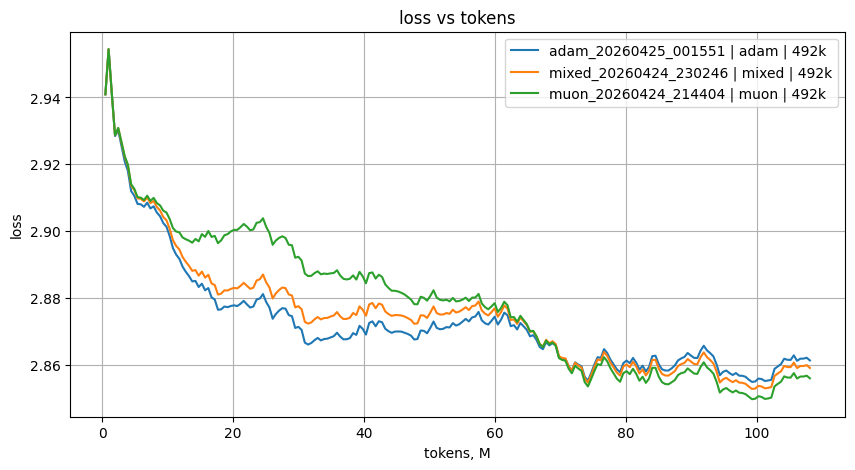
\includegraphics{report/attachments/Pasted image 20260427104850.png}
\emph{fig.~1 - 492k effective batch, 5e-5 AdamW lr, 1e-3 Muon lr, wd =
0.01, cosine annealing with \textasciitilde5\% warmup tokens.} However,
after approximately 66M tokens and until the end of training, the trend
reverses. Muon achieves the lowest loss, while the Mixed configuration
remains intermediate between Muon and AdamW.
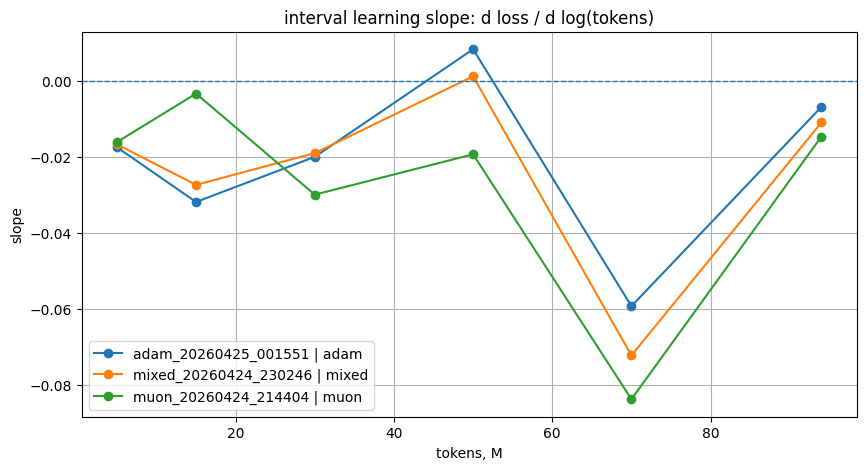
\includegraphics{report/attachments/Pasted image 20260427110942.png}
\emph{fig.~2 - learning rate slope display for Experiment 1}

For the second experiment, the effective batch size was reduced to 82k
tokens per update, increasing the number of update steps while keeping
all other settings unchanged. The goal was to evaluate whether Muon
scales effectively under a higher update frequency. In this run, a much
more pronounced post-warmup ``hill'' is observed compared to both the
AdamW baseline and the previous large-batch experiment. Immediately
after the warmup phase, Muon and Mixed show a stronger increase in loss.
However, similarly to the first experiment, Muon begins to close the gap
with AdamW and Mixed as the learning rate decreases.
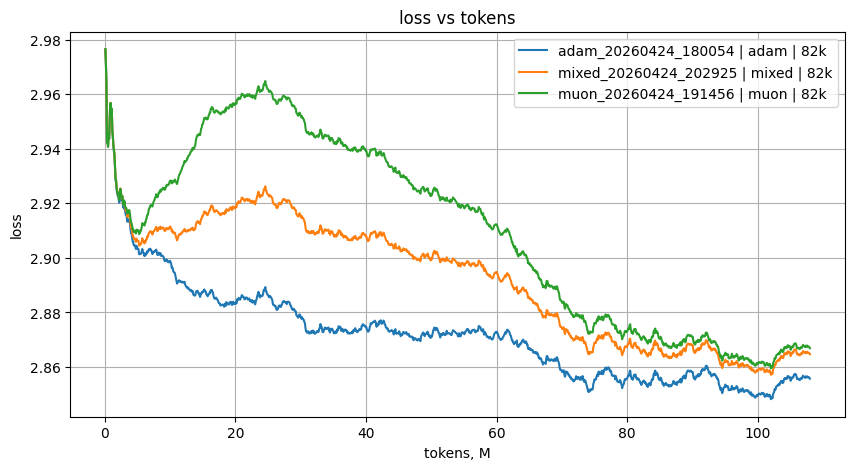
\includegraphics{report/attachments/Pasted image 20260427105822.png}\emph{fig.~3
- 82k effective batch, 5e-5 AdamW lr, 1e-3 Muon lr, wd = 0.01, cosine
annealing with \textasciitilde5\% warmup tokens.} Compared to Experiment
1, both Muon and Mixed exhibit a positive slope when exiting the warmup
phase. This behavior is likely caused by the higher update frequency,
which introduces noisier gradients.
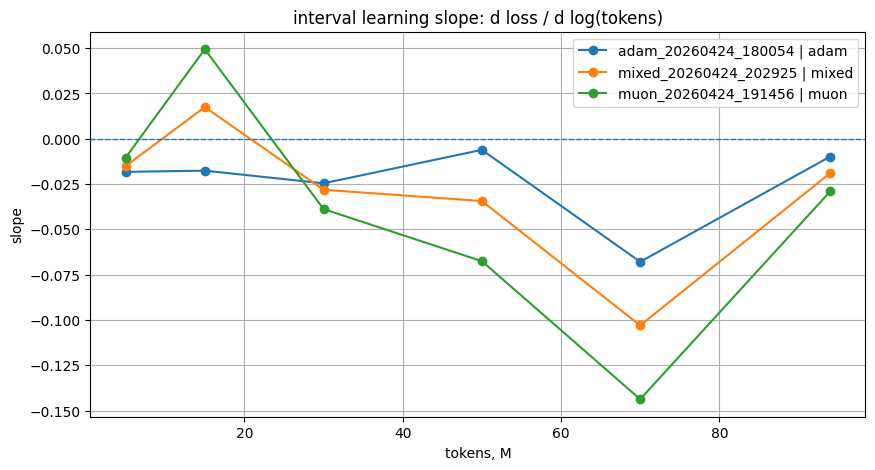
\includegraphics{report/attachments/Pasted image 20260427110718.png}
\emph{fig.~4 - learning rate slope display for Experiment 2} For the
final experiment, the Muon learning rate was reduced to
\(1 \times 10^{-5}\) and weight decay was set to \(0.0\), while keeping
the effective batch size at 82k tokens per update. The goal was to
stabilize Muon by reducing the magnitude of its updates. In this run,
the post-warmup spike is significantly reduced compared to the previous
experiment. Muon follows a much smoother trajectory and stays closer to
the Mixed configuration, although it still remains above the AdamW
baseline.
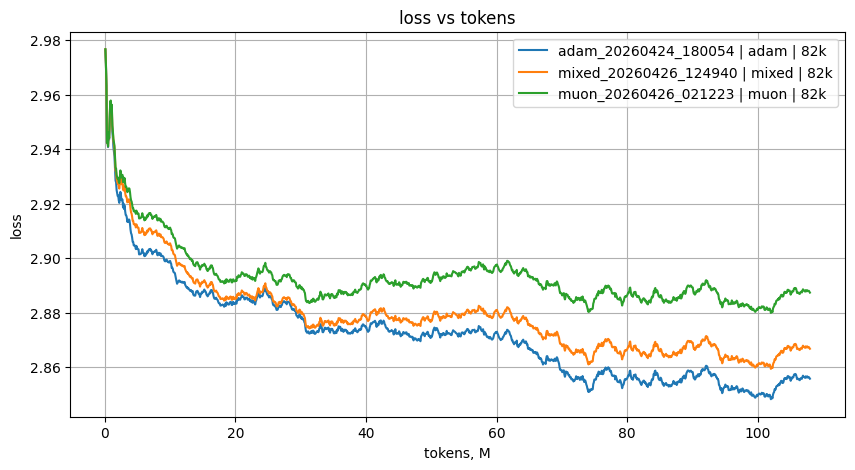
\includegraphics{report/attachments/Pasted image 20260427111756.png}
\emph{fig.~5 - 82k effective batch, 5e-5 AdamW lr, 1e-5 Muon lr, wd =
0.0, cosine annealing with \textasciitilde5\% warmup tokens.} The slope
analysis reflects improved stability. Muon no longer exhibits a strong
positive slope after the warmup phase, indicating that the transition is
less noisy. However, this comes at the cost of slower convergence: the
loss decreases more gradually, and Muon does not show the same rapid
recovery as in the higher learning rate setting. Overall, lowering the
learning rate and removing weight decay stabilizes Muon but reduces its
convergence speed, resulting in a more stable yet less competitive
optimization behavior compared to the baseline configurations.
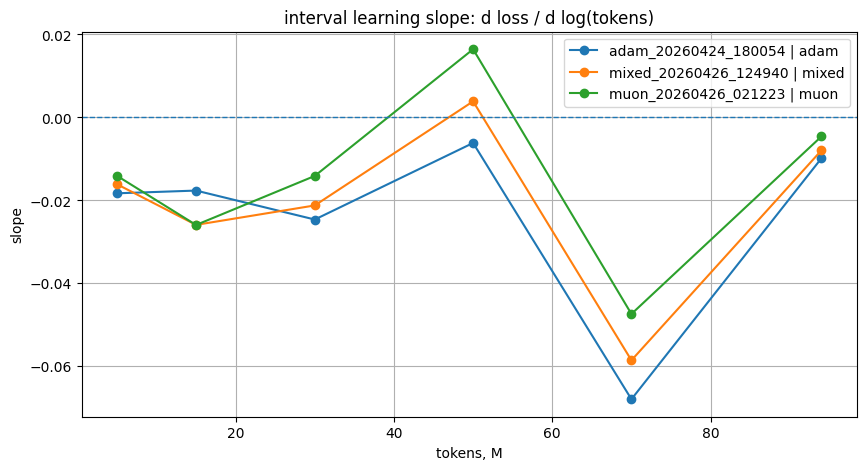
\includegraphics{report/attachments/Pasted image 20260427111803.png}\emph{fig.~6
- learning rate slope display for Experiment 2} \#\#\# 3. Evaluation
results The table shows performance on several downstream tasks for
different optimizer setups.\\
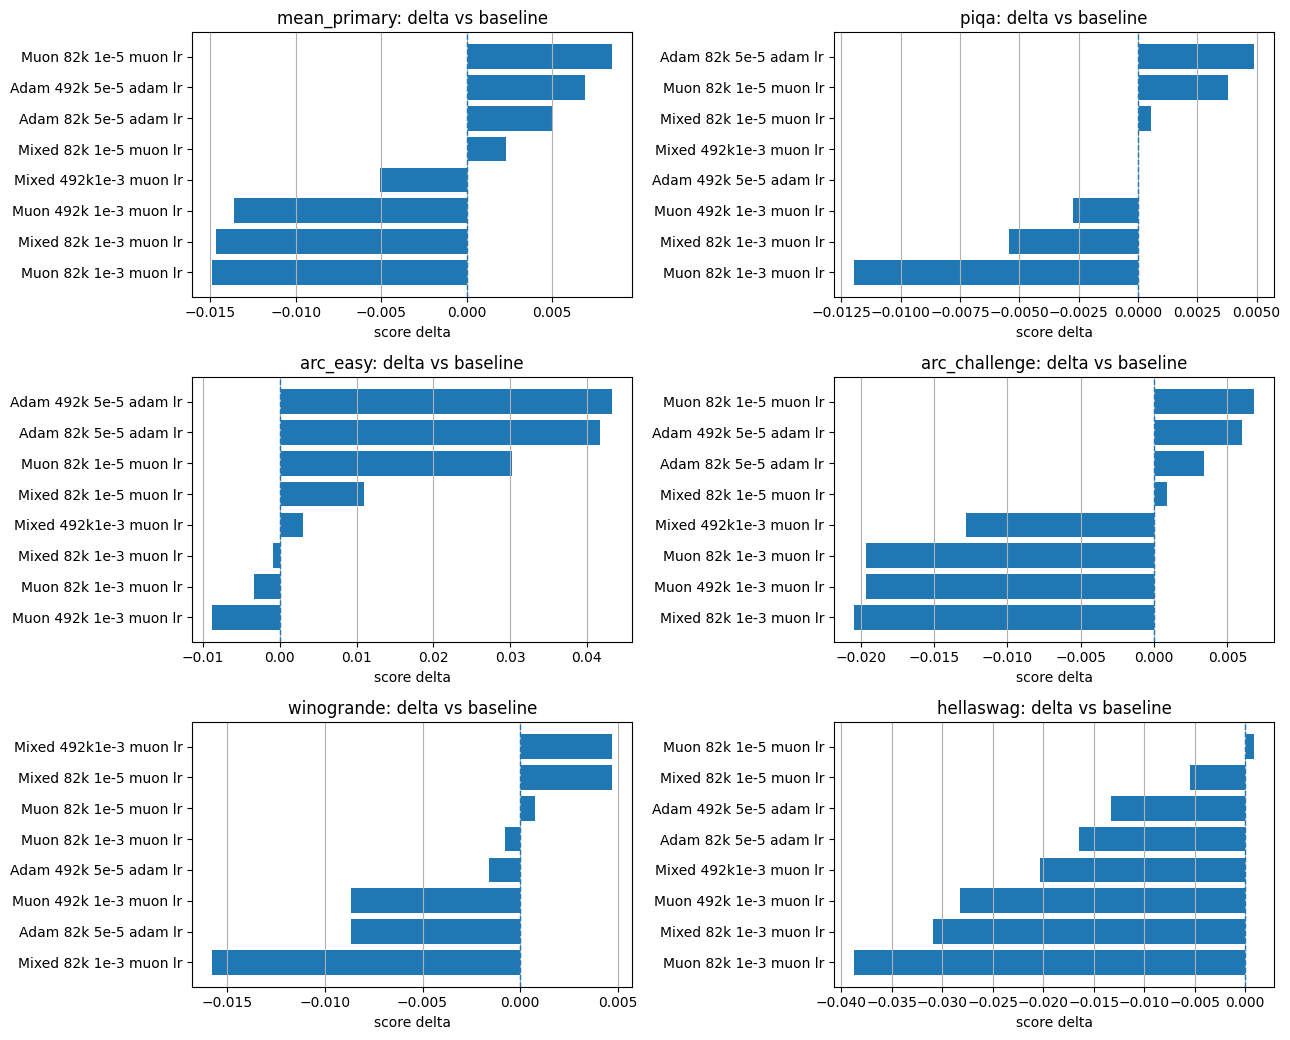
\includegraphics{report/attachments/Pasted image 20260427114520.png}
\emph{fig.~7 - evaluation results} The best overall results are achieved
by the final \textbf{Muon} run (with lower learning rate). It performs
at the top or near the top on most tasks. In particular:\\
- On \textbf{HellaSwag}, Muon achieves the highest score.\\
- On \textbf{PIQA} and \textbf{ARC-Challenge}, Muon is very close to the
best results.\\
- On \textbf{ARC-Easy}, \textbf{AdamW} remains slightly better.\\
- On \textbf{Winogrande}, \textbf{Mixed} configurations show competitive
or slightly better results. A key observation is the difference between
early and final runs:\\
- Earlier Muon runs with higher learning rate show worse results across
most tasks.\\
- After reducing the learning rate, Muon becomes much more stable and
improves consistently across all benchmarks.\\
Mixed configurations behave more conservatively:\\
- They are usually more stable than aggressive Muon setups,\\
- but do not reach the same peak performance as the best Muon run.\\
AdamW remains a strong and stable baseline:\\
- It performs consistently well across all tasks,\\
- and is especially strong on ARC-Easy.\\
Overall, Muon can outperform AdamW, but only when properly tuned. With
high learning rates, it tends to hurt generalization, while lower
learning rates make it competitive or better than the baseline. \#\# 3.
Resource efficiency analysis The first plot shows optimizer step time as
a percentage of the total step time. AdamW introduces very low overhead
in all configurations, typically staying below 1\%. In contrast, Muon
adds noticeable overhead due to the additional Newton--Schulz
iterations.
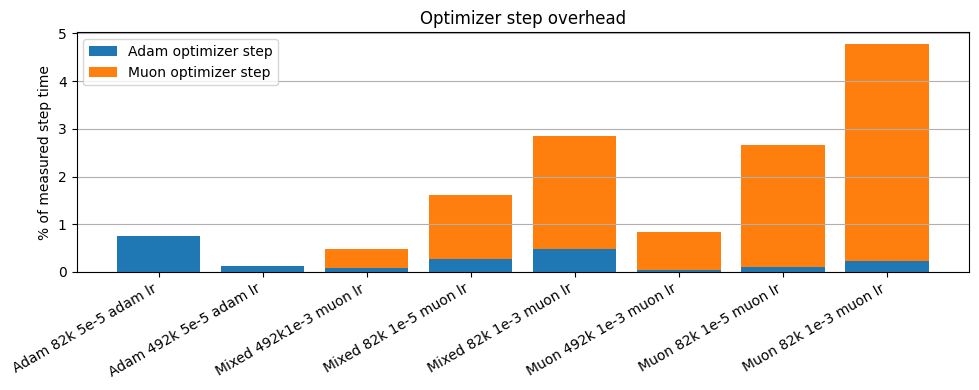
\includegraphics{report/attachments/Pasted image 20260427115756.png}
\emph{fig.~8 - optimizer step overhead} This overhead depends on the
setup: with large batch sizes it remains relatively moderate, while with
smaller batches it becomes significantly higher, reaching up to around
5\% in the most expensive case. This indicates that Muon is more
efficient when the forward and backward passes dominate computation, and
less efficient when optimizer cost becomes a larger fraction of the
step.
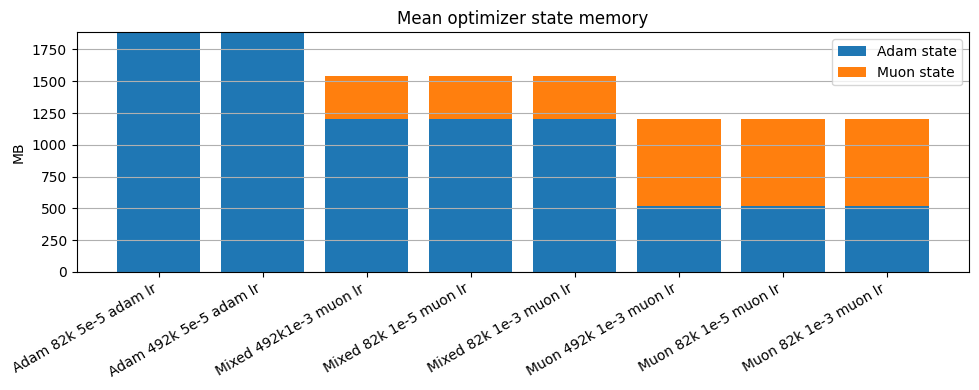
\includegraphics{report/attachments/Pasted image 20260427114533.png}
\emph{fig.~9 - optimizer memory usage} The second plot shows optimizer
state memory usage. AdamW consistently has the highest memory
consumption because it stores both first and second moment estimates for
all parameters. Muon requires substantially less memory, since it does
not maintain full moment statistics in the same way. Mixed
configurations fall between the two, reflecting the proportion of
parameters handled by each optimizer.\\
Overall, Muon provides a clear reduction in memory usage compared to
AdamW, typically by a factor of two to three, but this comes at the cost
of increased computation time per step. AdamW remains the most
computationally efficient, while Mixed configurations offer a compromise
between memory savings and computational overhead.

\end{document}
